\chapter{Background Research}\label{ch:backgroundresearch}
This chapter introduces the theories about augmented reality and human depth perception on which this project is based, as well as presents some reflections about the relation between the two. Lastly, a description of the state of the art provides some examples of existing systems with similar goals as those this project aims toward.

\section{Visual Depth Perception Within Humans}
Mathematical depth is to be thought of as the third dimension (first and second being length and width respectively). Depth is measured as the distance between two points in a vertical upward/downward and horizontal inward/outward direction depending on the objects of attention as well as angle of view (AOW) \cite{Gale}. Perception on the other hand defines the brain’s ability to sense and be aware of object’s existence through one or more of the five human senses: Hearing, smell, taste, touch, and vision. Of these the sense of vision --- primarily processed in the brain’s occipital lobe based on signals received from photoreceptors on the eyes’ retina registering the spatial, temporal, and chromatic components of light \cite{Spector2003} --- is considered the primary but not solemn sense for perceiving depth. As \textit{The Gale Encyclopedia of Science} states: \textit{“While depth perception results primarily from our sense of vision, our sense of hearing also plays a role.”} \cite{Gale}. Research with infants has further revealed that the ability to perceive depth visually within humans exist from as early on as two month of age \cite{Gale}. Thus it follows that visual depth perception within humans can be defined as the ability of humans with normal functioning eyes that follows the age of two month to use sight to see in three dimensions and estimate the spatial distances of objects from oneself and from each other.

\subsection{Depth cues}
For the brain to determine an object’s location in space and its relation to other objects certain estimates referred to as cues are used. Overall the cues can be separated into one of two types, namely monocular and binocular cues which are based on single eye and two eye information respectively. Furtheron, the monocular cue can be subdivided into pictorial cues and non-stereoscopic cues. To the pictorial cues belongs: Interposition, shading and lighting, aerial perspective, elevation, linear perspective, texture gradients, and retinal size, while the non-stereoscopic cues consist of motion parallax and accommodation. Meanwhile, members to the binocular cues are convergence and retinal disparity \cite{Gale}. 

\subsubsection{Monocular Depth Cues}
The following explains the aforementioned cues connected to monocular vision, meaning that these cues requires access to information from only one eye in order to be perceived.

\textit{Interposition} is when one object appears to be partially blocked by another object (as seen in Figure \ref{fig:cue0}), sometimes also referred to as occlusion or overlapping. During the image processing done by the brain this cue is used to determine which object should be perceived as the closest to the viewer since objects nearer the viewer tends to cover up parts of objects further behind \cite{Gale}.

\begin{figure}[h!]
   \centering
   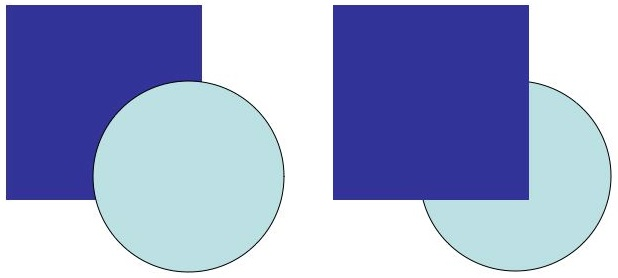
\includegraphics[width=0.7\textwidth]{figures/cue0.jpg}
   \caption{Interchange in occluded object to showcase the effect of interposition \cite{Heeger}}\label{fig:cue0}
\end{figure}

\textit{Shading and lighting} clues to the distance from the object to a light source as the surface closest to the light appears brighter than that of the surfaces further away which gradually darkens by the distance from the light source. Moreover, surfaces turned away from the light are perceived as dark progressing towards black the nearer they are to the light source. The viewer uses this to estimate whether to perceive the object as more convex or concave in shape \cite{Gale}. An example can be seen in Figure \ref{fig:cue1}.\pagebreak

\begin{figure}[h!]
   \centering
   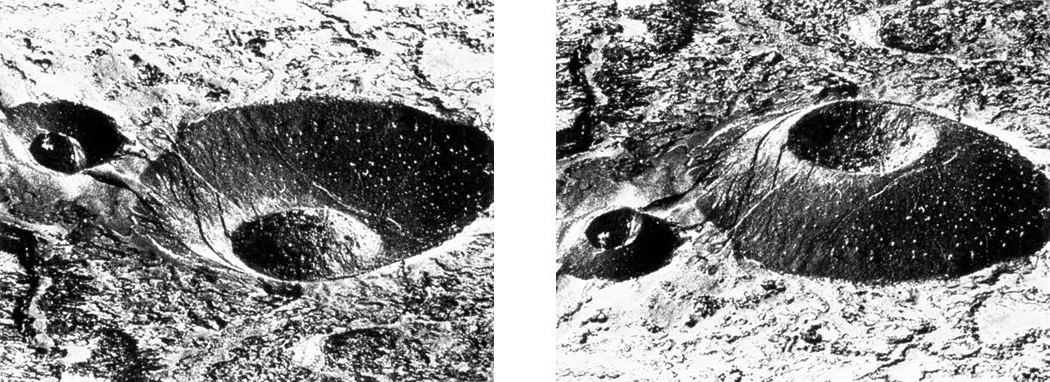
\includegraphics[width=\textwidth]{figures/cue1.jpg}
   \caption{Effects on the human depth perception by variations in shading and lighting \cite{Heeger}}\label{fig:cue1}
\end{figure}

\textit{Aerial perspective}, also known as \textit{atmospgeric perspective},  involves the sharpness of an object. From this it follows that the sharper an object is perceived by the eye, the nearer to the viewer the said object is interpreted to be, and the more blurred an object is perceived to be, the farther the distance seems between the object and the viewer. An example can be seen in Figure \ref{fig:cue2} The cause of this effect is the particles in the atmosphere e.g. water vapour and dust which either scatters or absorb light reflected by an object \cite{Gale}.  

\begin{figure}[h!]
   \centering
   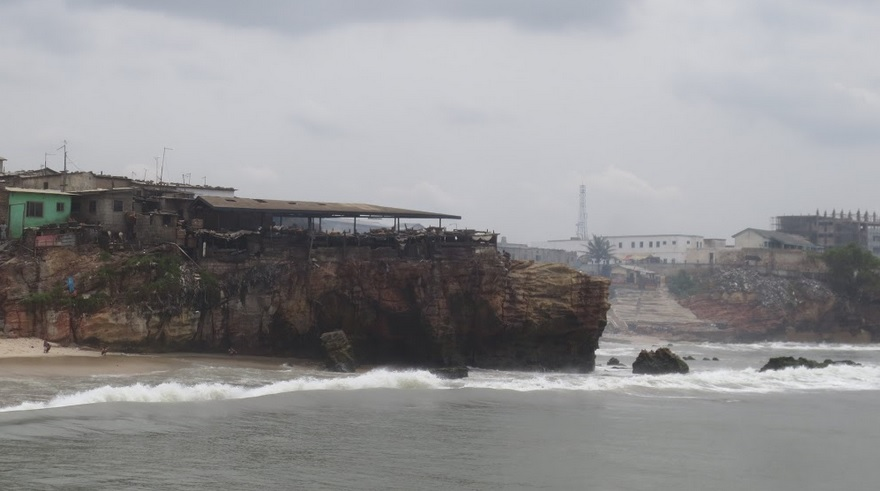
\includegraphics[width=\textwidth]{figures/cue2.jpg}
   \caption{Example of aerial perspective --- the buildings to the left are closer than the buildings to the right}\label{fig:cue2}
\end{figure}

\pagebreak
\textit{Elevation} considers the eyes’ placement of an object in correlation to the horizontal line, as can be seen in Figure \ref{fig:cue3}. Here the horizon (horizontal line, Figure \ref{fig:cue3}) is observed as either higher (foreground 1, Figure \ref{fig:cue3}) or lower  (foreground 2, Figure \ref{fig:cue3}) than that of the foreground. Thus objects placed near to the horizontal line is perceived as being in the distance in contrast to objects located near either the upper or lower outline of the visual field which are perceived to be nearer the viewer \cite{Gale}.   

\begin{figure}[h!]
   \centering
   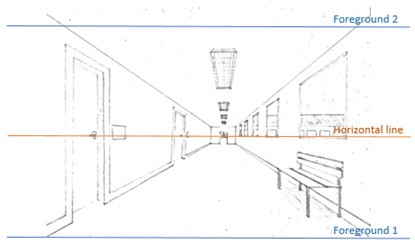
\includegraphics[scale=0.8]{figures/cue3.jpg}
   \caption{An example of elevation}\label{fig:cue3}
\end{figure}

\textit{Linear perspective} is the correlation occurring between the decrease in an object’s size and separating spaces on the retina when repeatedly lined up along a line and the perceived increase in distance from the point of view (POW) until the vanishing point is reached where the object cease to be visible, as can be seen in Figure \ref{fig:cue4} \cite{Gale}.

\begin{figure}[h!]
   \centering
   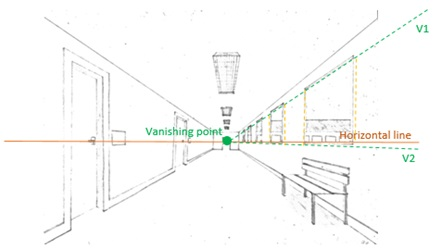
\includegraphics[scale=0.8]{figures/cue4.jpg}
   \caption{An example of linear perspective}\label{fig:cue4}
\end{figure}

\textit{Texture gradients} concerns the affection of texture perception by an increase in distance whereto it follows that by increased distance the size of elements that make up the surface texture appear to be smaller while the distance between said elements seems to decrease, as seen in Figure \ref{fig:cue5} \cite{Gale}.

\begin{figure}[h!]
   \centering
   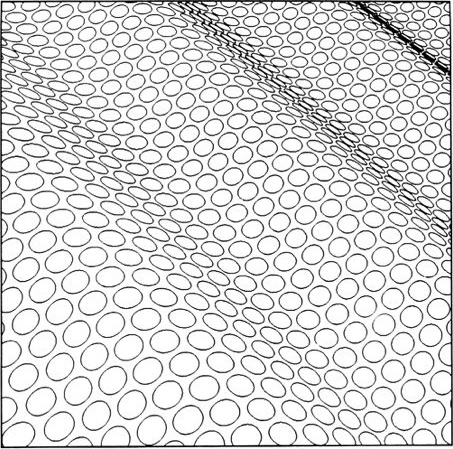
\includegraphics[width=0.4\textwidth]{figures/cue5.jpg}
   \caption{Texture gradient \cite{Heeger}}\label{fig:cue5}
\end{figure}

\textit{Retinal size} considers the brains automatically distinguish between an object being distant or near, interpreted based on the retinal image recognition of an object as small or large respectively, utilised in case of the absence of additionally visible cues to suggest the opposite. Thus, as it can be seen in Figure \ref{fig:cue6} the dotted arrow A, although having the same size as the arrow B, looks larger when comparing the projections of A and B on the retina, and hence it is considered to be nearer. However, as it is to be seen from the two airplanes in Figure \ref{fig:cue7} this method for distinguishing distance only applies for objects of the same size since a larger object located farther away may look the same size on the retina if compared to a nearer small object \cite{Gale}.

\begin{figure}[h!]
   \centering
   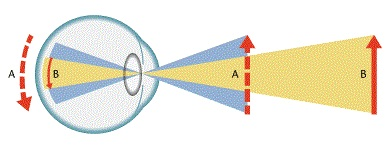
\includegraphics[scale=0.7]{figures/cue6.jpg}
   \caption{Retinal size used to infer distance \cite{Perslides}}\label{fig:cue6}
\end{figure}

\begin{figure}[h!]
   \centering
   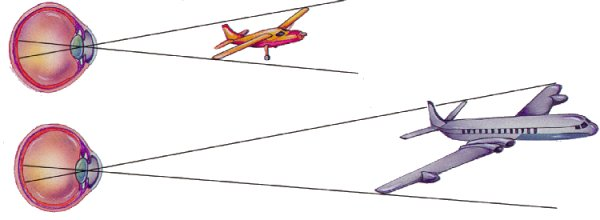
\includegraphics[scale=1]{figures/cue7.jpg}
   \caption{Retinal size, wrong interpretation of reality \cite{Psych}}\label{fig:cue7}
\end{figure}

\pagebreak
\textit{Motion Parallax} is the perception of apparent motion of two stationary objects with relative different distances to the viewer (located respectively in front of and behind of the viewer’s fixation point) caused by changes in the viewer’s position. This reasons in the movement of the eyes in relation to the spatial environment, because whenever a person move, the images projected by objects located at different distances as a result of said movement comes to move across the retina with different speed. To this it can be said that objects relative close to the viewer is perceived as moving at a higher speed when compared to objects located in the distance. Further on will the near object seem to be moving in the opposite direction as the viewer whereas the farther away object will be heading in the same direction as the viewer.  In addition to this it is also noticeable that distant objects seem to move smaller distances than that of objects near the viewer \cite{Gale} \cite{Shrestha2013} \cite{Skybrary}.

\begin{figure}
	\centering
	\begin{subfigure}[h!]{0.4\textwidth}
		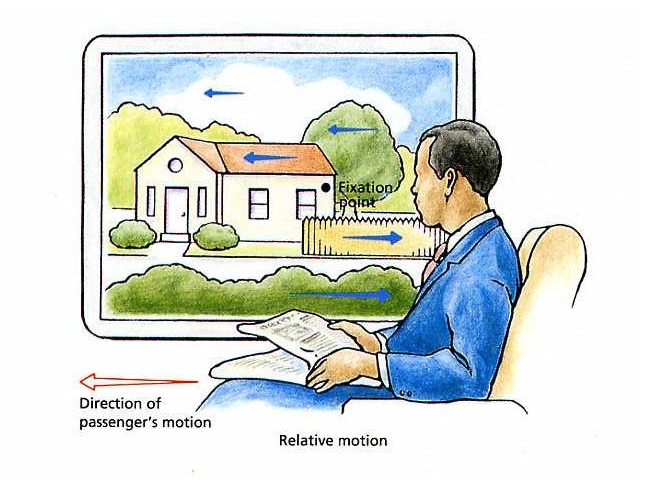
\includegraphics[width=\textwidth]{figures/cue8.jpg}
		\caption{Experiencing motion parallax \cite{Parallax0}}\label{fig:cue8}
	\end{subfigure}
	\begin{subfigure}[h!]{0.4\textwidth}
		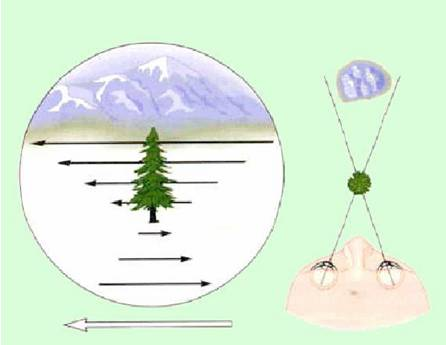
\includegraphics[width=\textwidth]{figures/cue9.jpg}
		\caption{Motion parallax explained \cite{Skybrary}}\label{fig:cue9}
	\end{subfigure}
	\caption{Illustrations demonstrating motion parallax}
\end{figure}

\begin{figure}[h!]
   \centering
   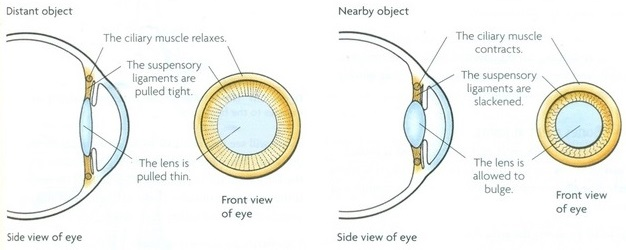
\includegraphics[width=0.8\textwidth]{figures/cue10.jpg}
   \caption{Accommodation, left: Distant focused lens, right: Near focused lens \cite{Biology2014}}\label{fig:cue10}
\end{figure}

\textit{Accommodation} is the physiological changes happening to the lens’ curvature to sharpen the retinal images of near and far objects. In order to have the eye focus on a distant object the lens have to flatten (Figure \ref{fig:cue10}, left). Meanwhile, to focus on near objects the lens becomes more of a curve (Figure \ref{fig:cue10}, right). These changes in the lens’ curvature are controlled by the ciliary muscle which seemingly sends signals as feedback to the brain about alterations in the muscle tension that may assist in determining the distance to the object \cite{Gale}.

In addition to monocular cues comes the semi-cue: Familiarity which is used in other sections of human’s visual processing as well. This takes as its starting point an individual’s previous experience with the spatial characteristics of various objects and contributes to determine the distance to the object thereby assisting in the spatial perception \cite{Gale}

\subsubsection{Binocular Depth Cues}
This will describe the two cues connected to binocular vision which means that the cues requires access to information from both eyes in order to be perceived.

\textit{Convergence} takes into consideration the eyes’ propensity to rotate inward toward each other in a coordinated manner in furtherance of an effectively focus on objects close to the eyes. In opposition to this the focus on distant objects have the eyes move outward toward the temples. However, changes in convergence cease to befall when an object exceeds the approximately distance of six metres from the eyes. Here the eye pupils reaches a point where they are essentially parallel to each other and cannot move any further away. It seems that the resulting muscular tension changes in the eye muscles that are required to cause these convergent eye movements in order to focus on near and far objects provide feedback to the brain about the depth or distance \cite{Gale}.

\begin{figure}[h!]
   \centering
   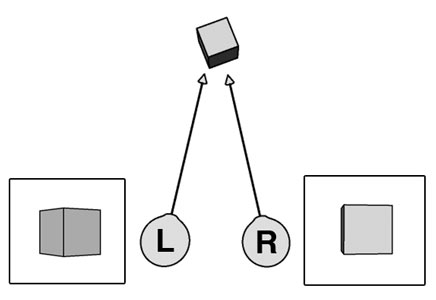
\includegraphics[width=0.4\textwidth]{figures/cue11.jpg}
   \caption{Example of retinal disparity between  left and right eye \cite{Retina}}\label{fig:cue11}
\end{figure}

\begin{figure}[h!]
   \centering
   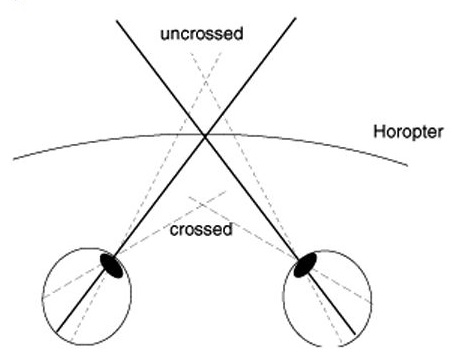
\includegraphics[width=0.4\textwidth]{figures/cue12.jpg}
   \caption{Distinction between crossed and uncrossed disparity \cite{Heeger}}\label{fig:cue12}
\end{figure}

\textit{Retinal disparity} is caused as a result of humans’ laterally arrangement of the two eyes which provides a positional difference (an interocular distance of 60 to 65 mm). This positional difference let us see the world from two slightly different points of perspective. Disparity here occurs where a singled out object in the images constructed in each of the two eyes do not stimulate corresponding points on the respective retinae hereof the name: ‘retinal disparity’ (or binocular disparity).  Mainly these differences happens in the relative horizontal position of objects which is why they are also sometimes referred to as horizontal disparity, and is defined by McCoun and Reeves as: \textit{“the difference in position of corresponding points between images in two eyes”} \cite{McCoun2010}.

Set into relation to the convergence of the eyes when focused on a fixed point (FP), retinal disparity can moreover be classified as either crossed or uncrossed. From FP an imaginary 3D surface called the horopter can be made consisting of all the positions in the two retinae that correspond (Figure \ref{fig:cue12}). If a point is perceived as within the range closer than that of FP it in general has lines of sight that cross in front of the horoptor. Such an occurrence is called a crossed disparity (Figure \ref{fig:cue12}). Alternatively do any point positioned beyond the range of FP typically have lines of sight meet behind the horoptor, resulting in the lines not crossing each other before this point, hence the name uncrossed disparity (Figure \ref{fig:cue12}) \cite{McCoun2010}.

When the subtle differences between the retinal images from the eyes are forwarded to the brain neural processes merge them such that they become a single percept. This produces a series of smaller disparities that permits a specific form of depth perception known as stereopsis, and its perceived visual result is a 3D image \cite{Parker2007}.

\subsection{Reflections Upon Human Depth Perception in The Context of AR}
A major part of an AR system is to have the digital 2D overlay image appear as an integrated part of the real world environment generated by the real time video transmission, and since any camera imitates the eye’s retina in the way it produces its images. Thus it befalls that the retina based cues for depth perception in the human eye also applies to a camera’s way of processing the sense of depth in an image.

\begin{figure}[h!]
   \centering
   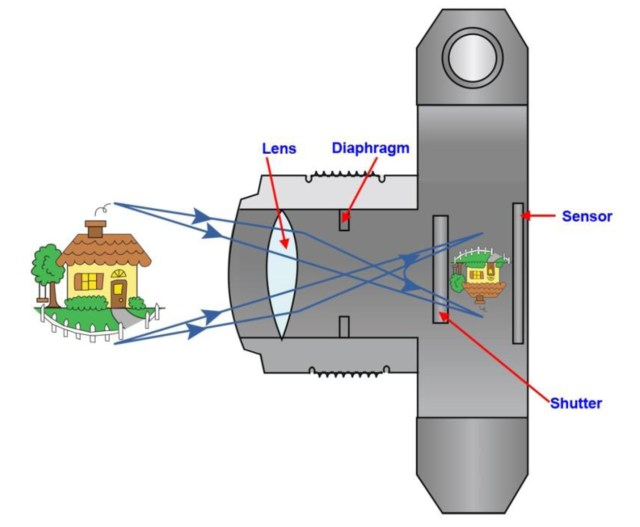
\includegraphics[width=0.5\textwidth]{figures/camera.jpg}
   \caption{Camera image production \cite{Camera}}\label{fig:camera}
\end{figure}

To this it has to be added that unless two cameras are used to produce the image, one only have to consider the monocular depth cues, given that the binocular cues requires two eyes, or in this case two cameras, in order to be obtained. This further means that the pictorial depth cues becomes the primary source for integrating a digital AR overlay into a real time footage, because the non stereoscopic monocular depth cues relates to physical movement or changes in the eye muscles for which reason they are outside the AR system’s control.

\section{Augmented Reality}
As suggested by Madden in the book Professional Augmented Reality Browsers for Smartphones, AR is to be thought of as the opposite of Virtual Reality (VR). As Madden explains it: “Virtual reality immerses the user in a computer-generated world whereas AR combines the real world with computer graphics.” \cite{Madden2011}. Moreover, Madden points out that where it requires the user to acquire special equipment to experience VR, AR requires only a device able to capture the environment (e.g. a smartphone or tablet) as well as methods to experience the computer world typically in the form of an overlaying computer graphic in the camera window \cite{Madden2011}. Based on this, Madden defines AR as a technology which combines the real world with computer graphics, tracking and/or providing interaction with objects in real-time. Furthermore, AR provides recognition of images or objects, as well as delivering real-time context or data. By utilising this definition Madden allows technologies to be included that are not considered AR in the strictest interpretations e.g. AR browsers \cite{Madden2011}.

In relation to the above definition of AR, Madden makes a distinction between two tracking systems, namely tracking by markers and markerless tracking. The method of tracking by markers makes use of patterned images, which activate a certain action when recognised. Examples of markers are the fiduciary marker, Quick response codes (QR), and Microsoft Tags. Markerless tracking on the other hand works by tracking objects in the real world not using markers made for the purpose. An example of markerless tracking is facial recognition \cite{Madden2011}.

Approaches to mobile AR are mainly split into two paths, namely AR using location and orientation data to compute what is viewed, and AR using actual image content captured by a camera to compute what is viewed referred to as \textit{computer vision}.

As introduced by Madsen and Lal, Aalborg University, in the book Augmented Reality, chapter 2 \cite{Lal2010}, AR can be associated with three major challenges:

\begin{enumerate}
\item Camera tracking 
\item Handling occlusions
\item Illumination consistency
\end{enumerate}

The obstacle with camera tracking involves \textit{“matching position and orientation of the camera to the coordinate system of the scene”} \cite{Lal2010}, which deals with making sure the angle of the scene captured by the camera matches that of the virtual scene. Handling occlusions means \textit{“having sufficient 3D information of the real scene to handle occlusion between real and virtual geometry”} \cite{Lal2010}, so that real-world objects such as people walking by may occlude the virtual objects. Lastly, illumination consistency deals with the problems of \textit{“having sufficient knowledge of the real scene illumination to be able to render virtual objects with scene consistent illumination, including shadows”} \cite{Lal2010}. The latter of these three is especially important for creating visually credible AR in outdoor environments because of this scenario’s dynamically changing illumination.

\section{State of the Art}
Augmented reality can be used to various ends. The popular game Pokémon Go, which was released in the summer of 2016, includes an optional AR feature \cite{Pokemon}. However, AR has also been utilised for tourism. Feiner et al. (1997) developed a system which allowed users to access access information about a campus using an overlay interface \cite{Feiner1997}. Because of the age of this prototype, however, a bulky setup was required, including a backpack-worn computer and a head-mounted display. A prototype built by Fritz et al. (2005) uses a camera, binoculars and internal sensors to augment a video stream with graphical objects, such as information of a site, or visualisations of what a site looked like in the past \cite{Fritz2005}. A sketch of this prototype is seen in Figure \ref{fig:binoculars}.

\begin{figure}[h!]
    \centering
    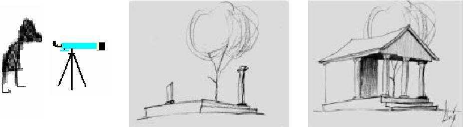
\includegraphics[scale=0.7]{figures/binoc.png}
    \caption{Sketch of Fritz et al.'s prototype (left), the unaugmented image (middle), and the augmented image (right) \cite{Fritz2005}}\label{fig:binoculars}
\end{figure}

While a majority of AR solutions for tourists are scientific prototypes, a few commercial products are available for mobile smartphones. Using apps such as Wikitude, users can experience several different types of AR experiences, as developers are able to upload their AR project to the platform. This allows various third-party stakeholders to utilise the app. A screenshot of Tripadvisor's use of the Wikitude platform can be seen in Figure \ref{fig:wikitude}. The app uses different input methods to load the AR experiences, such as GPS location, images, and QR-codes \cite{Wikitude}. It primarily functions as a platform for AR advertisements or similar commercial products.

\begin{figure}[h!]
    \centering
    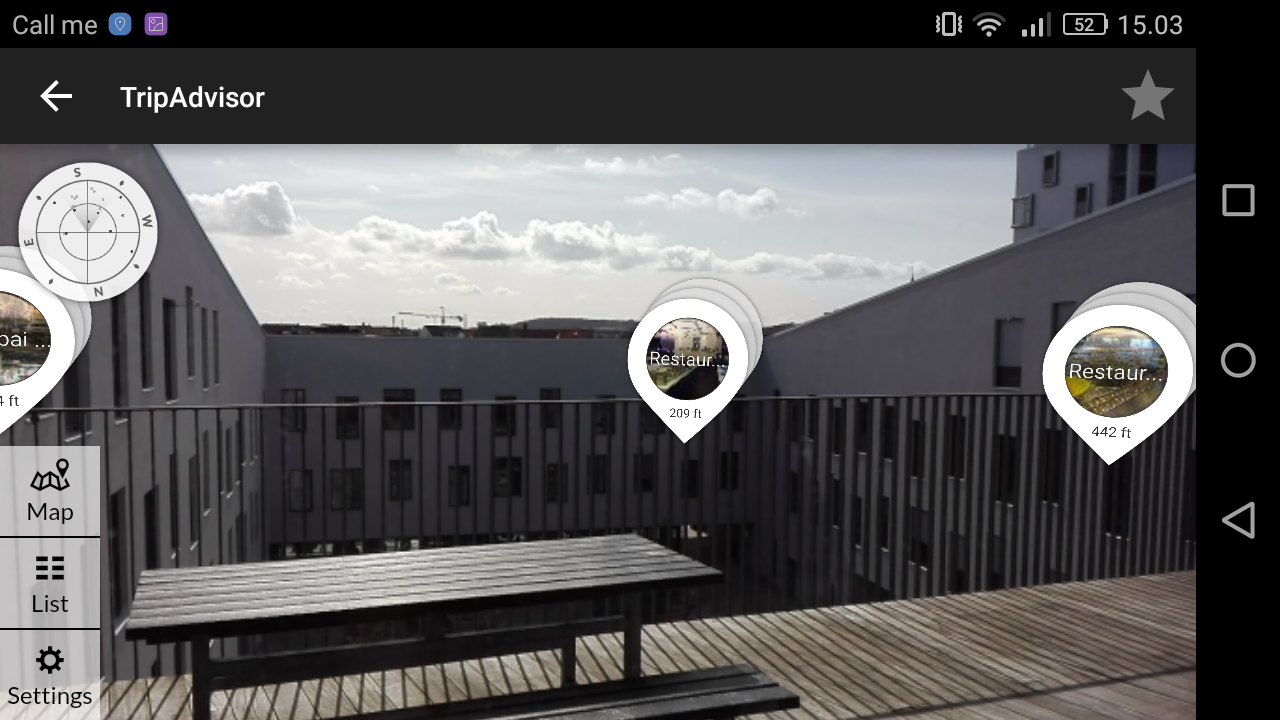
\includegraphics[width=0.65\textwidth]{figures/wikitude.png}
    \caption{Screenshot of the Wikitude app, as utilised by Tripadvisor}\label{fig:wikitude}
\end{figure}

The Yelp app, dedicated to reading and writing reviews of local restaurants, has an optional feature called \textit{monocle}, which allows users to see the average rating of nearby restaurants based on location \cite{Yelp}. A downside to this feature is that depending on the density of nearby restaurants, the screen may get quite cluttered, as can be seen in Figure \ref{fig:yelp}.

\begin{figure}[h!]
    \centering
    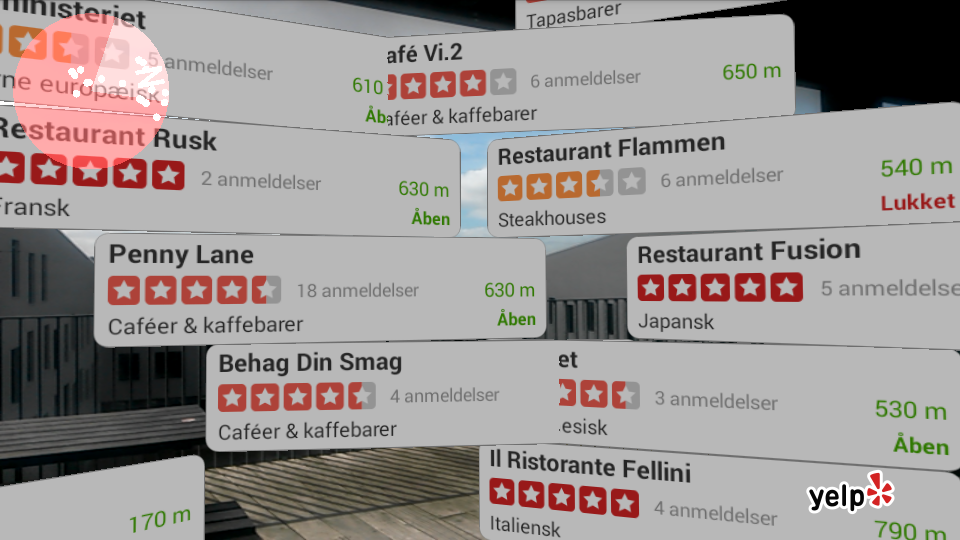
\includegraphics[width=0.65\textwidth]{figures/yelp.png}
    \caption{Screenshot of the Yelp monocle feature}\label{fig:yelp}
\end{figure}

%I am just commenting this out in case we need it
%Here is equation~\eqref{eq:esun}:

%\begin{equation}
%\label{eq:esun}
%E_{sun} = (\vec{n} \cdot \vec{s}) \times \_E_{sun}
%\end{equation}